% Ajout éditorial séparé du manuscrit original.

\chapter*{Ajout du transcripteur --- hors document original}
\addcontentsline{toc}{chapter}{Ajout du transcripteur --- hors document original}

\begin{quote}
\textit{Ce chapitre ne fait pas partie des Mémoires de Benoît Coste. C'est un
ajout du transcripteur, destiné uniquement à donner au lecteur un contexte
familial.}
\end{quote}

Il s'agit d'un schéma généalogique des ascendants et descendants directs du
couple Coste/Colomb.

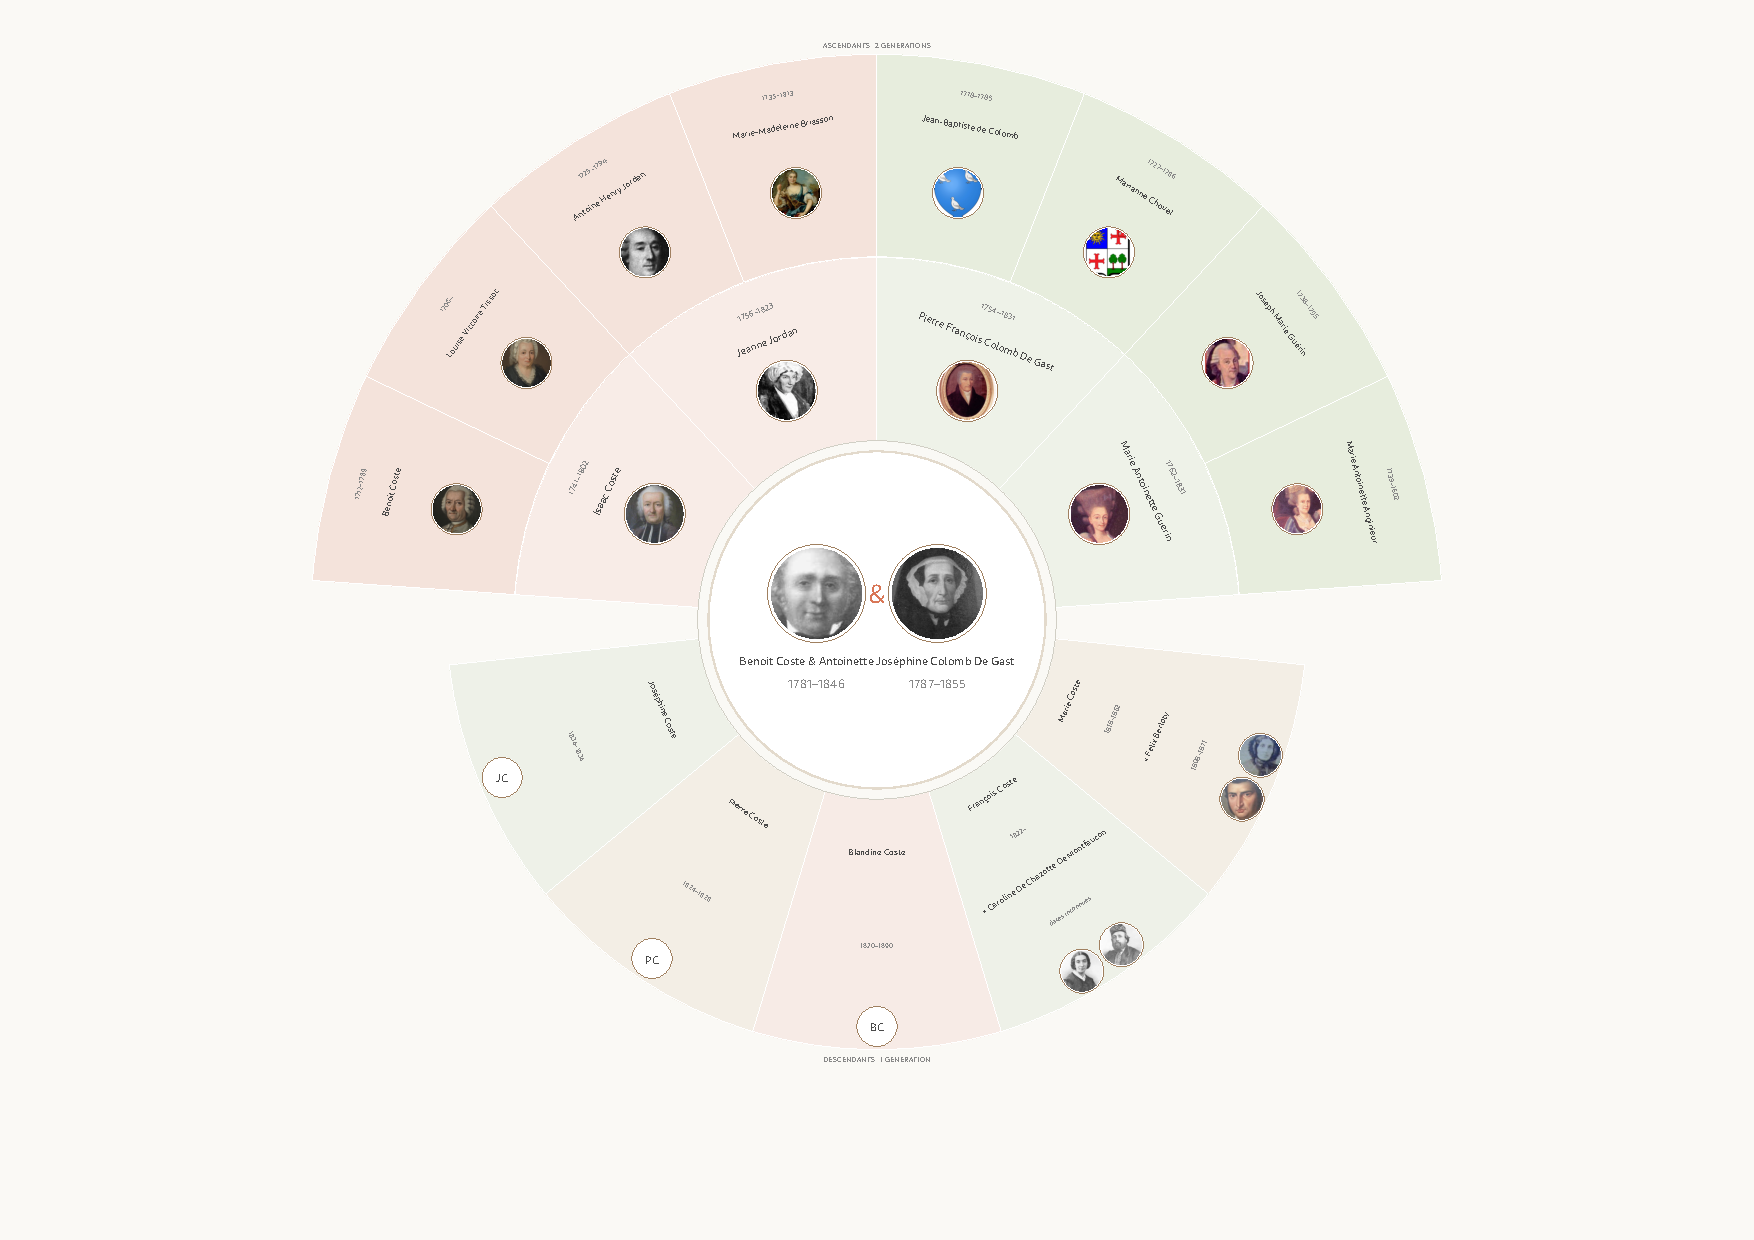
\includepdf[fitpaper]{genealogie/assets/arbre-benoit-coste-a4-overview.pdf}